
%%%%%%%%%%%%%%%%%%%%%%%%%%%%%%%%%%%%%%%%%%%%%%%%%%%%%%%%%%%%%%%%
\subsection{Prototype RGB-SPAD Camera Hardware}

% The laser operates at 450~nm with a pulse repetition rate of 25~MHz with a peak power of 450~mW and average power of 0.5~mW.
% \begin{figure}[t]
% 	\centering
%   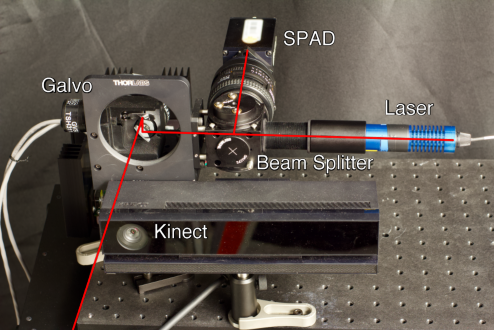
\includegraphics[width=0.5\columnwidth]{prototype_single_col.pdf}
%   \caption{Prototype scanning setup. The pulsed light from the laser travels
%     through a beam splitter before being guided by the galvo to the scene.
%     Returning light is measured by the single-pixel SPAD. The Kinect v2 RGB 
%     camera is used to capture the image used to generate the monocular depth estimate
%     (the depth camera is not used).}
%   \label{fig:prototype}
%   % \vspace{-0.5em}
% \end{figure}


As shown in Figure~\ref{fig:hardware}, our prototype comprises a color camera
(Microsoft Kinect v2), a single-pixel SPAD (Micro Photon Devices 100~$\mu m$ PDM
series, free-running), a laser (ALPHALAS PICOPOWER-LD-450-50), and a two-axis
galvanometer mirror system (Thorlabs GVS012). The laser operates at 670~nm with
a pulse repetition rate of 10~MHz with a peak power of 450~mW and average power
of 0.5~mW. The ground truth depth map is raster-scanned at a resolution of $512 \times 512$ pixels, and the single transient is generated by summing all of these measurements for a specific
scene. This allows us to validate the accuracy of the proposed histogram matching algorithm, which only uses the integrated single histogram, by
comparing it with the captured depth. To verify that our digitally aggregated scanned SPAD measurements match measurements produced by an optically diffused SPAD (see Figure~\ref{fig:hardware}(b,c)), we set up a slightly modified version of our prototype consisting of both scanned and optically diffused SPADs side-by-side. Additional details about the hardware prototype can be found in the supplement.


% show this in supplement
%The monocular depth estimate is calculated using the RGB image captured by the Kinect v2. The SPAD records temporal histograms with 4096 bins, each corresponding to a time window of 16~ps. The SPAD and laser are co-axially aligned using a beam splitter (Thorlabs PBS251). The full width at half maximum (FWHM) of the combined laser pulse width and SPAD jitter is about 70~ps, allowing the system to record depth maps with an accuracy of about 1~cm. A National Instruments data acquisition device (NI-DAQ USB-6343) provides synchronization signals for the galvos, SPAD, and laser. The ground truth depth map is raster-scanned at a resolution of $512 \times 512$ pixels, and the single-pixel, diffused SPAD measurement is generated by summing all of these measurements for a specific scene. This allows us to validate the accuracy of the proposed histogram matching algorithm, which only uses the integrated single histogram, by comparing it with the captured depth---\edit{such validation would not be possible if we were to capture measurements with an optically diffused SPAD.}

% show this in supplement
%\edit{To verify that our digitally aggregated scanned SPAD measurements match measurements produced by an optically diffused SPAD, we set up a slightly modified version of our prototype consisting of both scanned and diffused SPADs side-by-side. Details about this system can be found in the supplement. We then captured measurements of the simple scene shown in Figure~\ref{fig:hardware}(b) with both SPADs. The aggregated measurements from the scanned SPAD are shown alongside the optically diffused SPAD's measurements in Figure ~\ref{fig:hardware}(c). These results demonstrate that the two systems produce near equivalent measurements. Slight differences in their two histograms can be attributed to a baseline difference of about 10cm between the SPAD positions. That is, they observe scene from slightly different perspectives.}
	%NOTE:JUSTIFY USE OF DIFFERENT PROTOTYPE FOR RESULTS IN THE WILD WITH EYE SAFETY?} \edit{We show proof-of-concept results captured by this system in   Figure~\ref{fig:captured_diffuse_small}. For}

\begin{figure}[t]
	\centering
  \includegraphics[width=0.8\columnwidth]{hardware.pdf}
  \caption{(a) Prototype scanning setup. The pulsed light from the laser travels
    through a beam splitter before being guided by the galvo to the scene.
    Returning light is measured by the single-pixel SPAD. The Kinect v2 RGB 
    camera is used to capture the image used to generate the monocular depth estimate
    (the depth bccamera is not used). (b) Scene and (c) measurements for diffused and summed scanned mode. The observed
    counts in the diffuse mode match closely with the sum of the raster-scanned
    measurements.}
  \label{fig:hardware}
  % \vspace{-0.5em}
\end{figure}

We determined camera intrinsics and extrinsics for the Kinect's RGB camera and
the scanning system using MATLAB's camera calibration toolbox. 
The SPAD histogram and RGB image were captured from slightly different
viewpoints; we account for this in the SPAD histogram by shifting the 1D
transient according to the SPAD's offset from the RGB camera. We re-bin the
captured 1D transient for the indoor captured results
using Equation~\ref{eq:sid_bin_edges} with $K = 600$ bins, and $(\ell, u)=(0.4, 9.)$.
For the outdoor captured result, we use $K=600$ and $(\ell, u)=(0.4, 11)$.
%We use the camera extrinsics to Once the SPAD volume has been summed over the spatial dimensions, it is unclear
%how to warp the resulting 1D transient to the RGB camera's perspective (in a
%single-pixel flash LiDAR setup, the $512 \times 512$ ground truth data is not
%available). However, we do shift the 1D transient by the $z$ displacement
%between the SPAD and the RGB camera to partially account for this.

%% \textcolor{red}{Mark, please write a short paragraph on calibration details, including any warping of the SPAD histograms you did to compensate for the offset in camera and SPAD position.}
%
%Missing:
%%
%\begin{itemize}
%\item RGB resolution used for MDE
%\item do we also have Kinect depth maps for comparison? (yes) kinect resolution: RGB is 1920x1080 and depth camera is 512x424
%\end{itemize}

%%%%%%%%%%%%%%%%%%%%%%%%%%%%%%%%%%%%%%%%%%%%%%%%%%%%%%%%%%%%%%%%
\subsection{Experimental Results}
\begin{figure}[t]
	\centering
	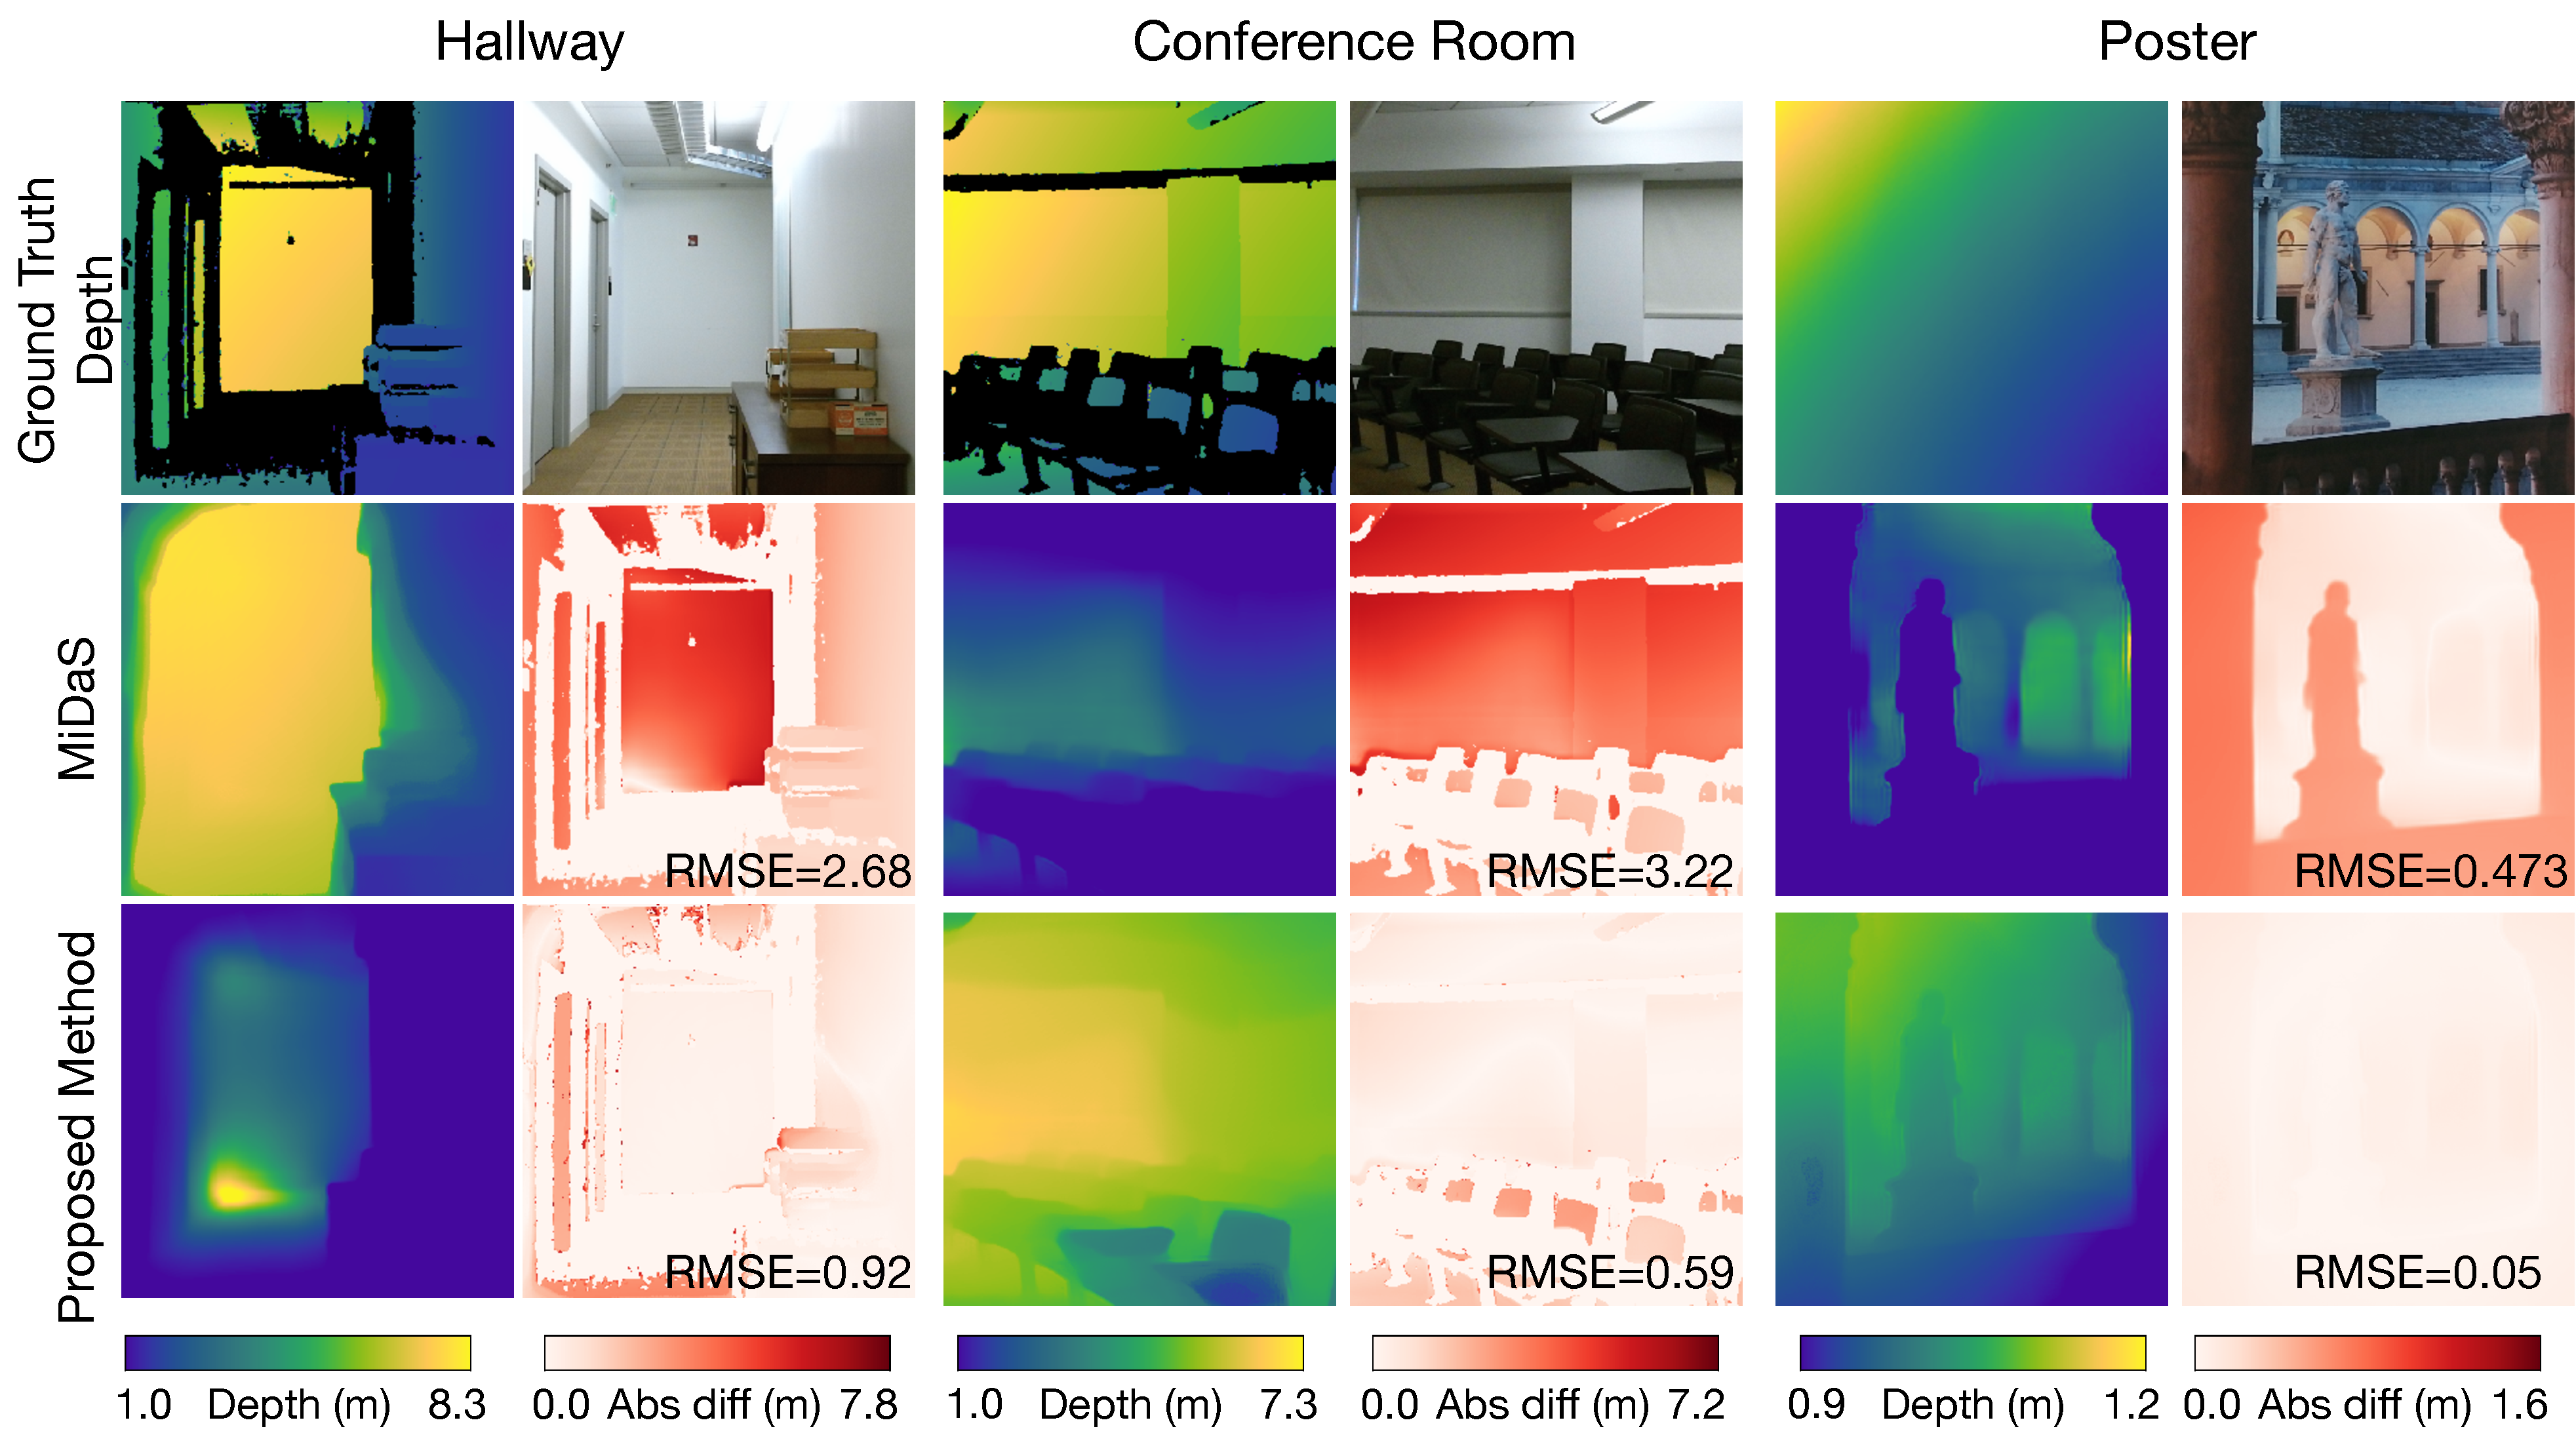
\includegraphics[width=\columnwidth]{captured.pdf}
	\caption{Experimental results. For each scene, we record a ground truth depth
    map that is raster-scanned with the SPAD (upper left subimages), and an RGB
    image (lower left). A monocular depth CNN predicts an initial depth map (top
    middle), which is corrected with the digitally aggregated SPAD histogram using the
    proposed method (top right), as shown by the error maps and root mean
    squared error (RMSE) for each example (lower center, right). The CNN is
    confused when we show it a photograph of a poster (bottom scene); it
    incorrectly predicts the depth of the scene depicted on the flat print. Our
    method is able to correct this error.}
	\label{fig:results_captured}
\end{figure}

\begin{figure}[t]
	\centering
  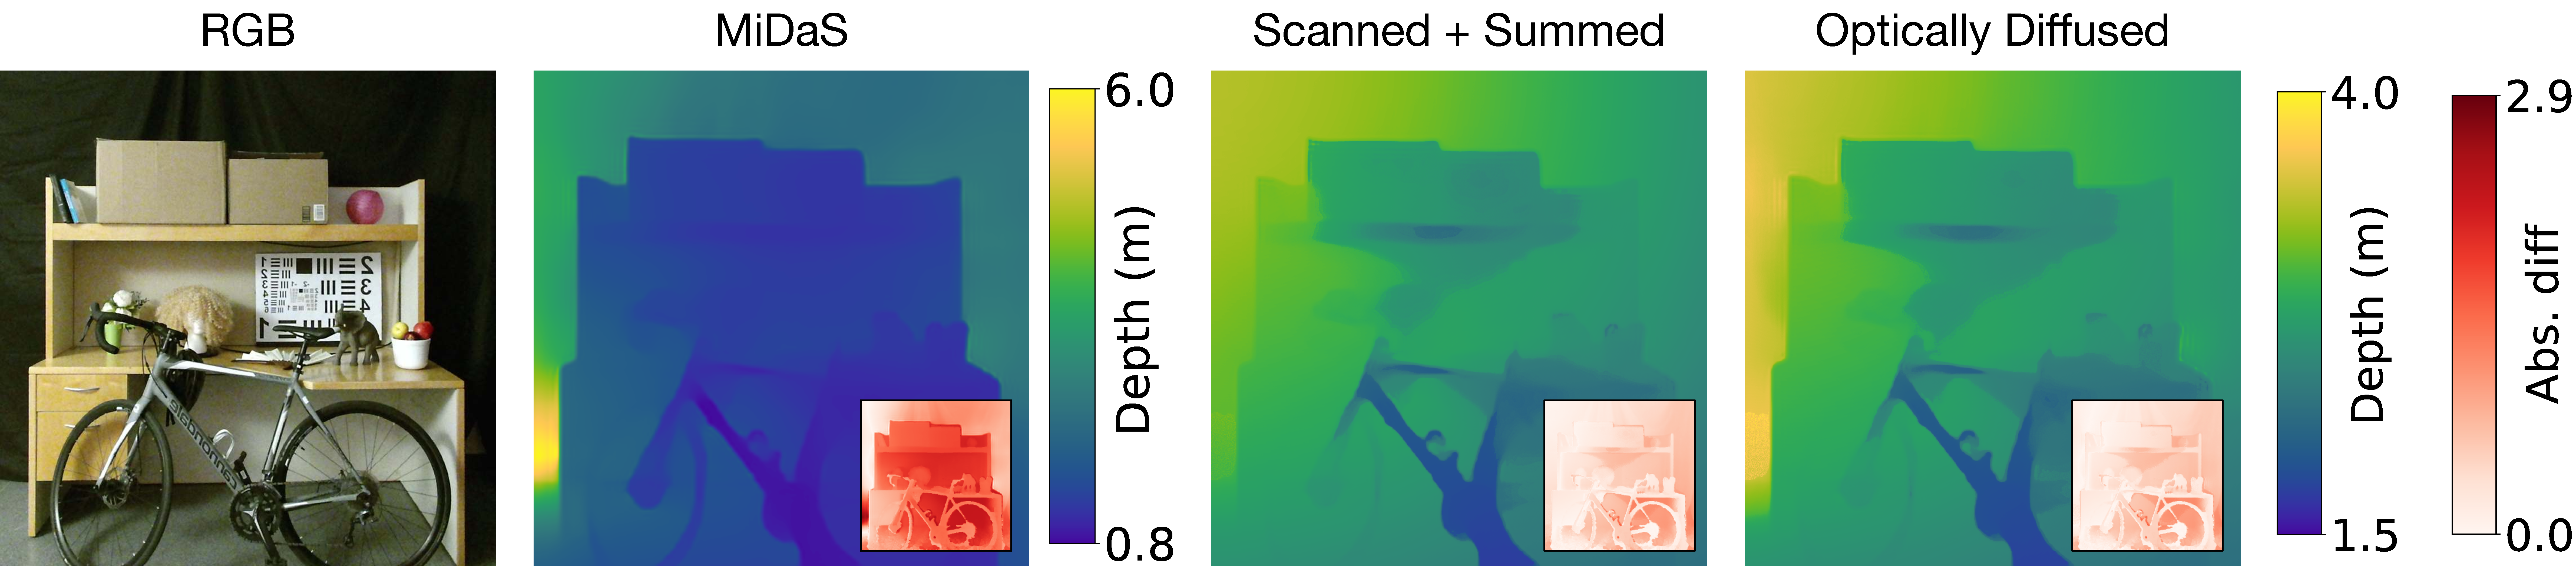
\includegraphics[width=\columnwidth]{captured_diffuse_small.pdf}
  \caption{Captured result comparing the direct output of the MiDaS MDE and depth maps corrected by our method using the digitally aggregated transient of the scanned SPAD (center right) and a single transient captured by an optically diffused SPAD and laser (right). Both of these approaches result in very similar results and both are significantly better than the output of the MDE, as shown by the error maps in the insets. The diffused SPAD results are captured at $\sim$25mW laser power indoors.
			%The resulting corrected depth maps from both scanning and summing transient measurements and diffusing the laser illumination are very similar qualitatively and quantitatively.
		}
  \label{fig:captured_diffuse_small}
  % \vspace{-0.5em}
\end{figure}

Using the hardware prototype, we captured a number of scenes as shown in
Figures~\ref{fig:results_captured},~\ref{fig:captured_diffuse_small}, and in the supplement. We crop the RGB image
to have dimensions that are multiples of 32. For DORN only, we further
downsample the image to a resolution of $353 \times 257$. We then feed this RGB
image into the monocular depth estimation algorithm. In
Figure~\ref{fig:results_captured} we show a subset of the scenes we captured and
processed with MiDAS~\cite{Lasinger:2019}, which achieved the best results among
the depth estimators we tested. Additional scenes, also processed with other MDE
approaches, including DenseDepth~\cite{Alhashim2018} and DORN~\cite{Fu2018}, are
included in the supplement. The ground truth depth is captured with the scanned
SPAD, as described above, and regions with low signal-to-noise ratio are masked
out (shown in black).

In the first two examples, the ``Hallway'' and ``Conference Room'' scenes, we
see that the monocular depth CNN estimates the ordinal depth of the scene
reasonably well. However, the root mean squared error (RMSE) for these two
scenes is relatively high ranging from 2.6--3.2~m (see red/white error maps in
Fig.~\ref{fig:results_captured}). The proposed method using a single diffused
SPAD measurement corrects this systematic depth estimation error and brings the
RMSE down to 0.6--0.9~m. The ``Poster'' scene is meant to confuse the CNN---it
shows a flat poster with a printed scene. As expected, the CNN predicts that the
statue is closer than the arches in the background, which is incorrect in this
case. The proposed method uses the SPAD histogram to correctly flatten the
estimated depth map.

Figure~\ref{fig:captured_diffuse_small} shows the RGB image of a scene along with the monocular depth estimate computed by MiDaS and depth maps corrected by our method using both the digitally aggregated transients from the scanned SPAD and the single optically diffused measurement, which are very similar. %Both scanned \& summed and diffused transients result in very similar depth maps and both are significantly better than the raw output of the MDE. The transient measurements for this scene are shown in the supplement.

